% =====================================================================
% OPTION B — Big-numbers infographic
% A0 vertical (841 mm × 1189 mm). Bold colored bands, huge headline
% numbers, magazine-spread aesthetic. Built around the +0.99 reveal.
% =====================================================================
\documentclass[a0paper, portrait]{article}

\usepackage[paperwidth=841mm, paperheight=1189mm,
            top=0mm, bottom=0mm, left=0mm, right=0mm]{geometry}
\usepackage[T1]{fontenc}
\usepackage{lmodern}
\usepackage{microtype}
\usepackage{amsmath, amssymb}
\usepackage{tikz}
\usetikzlibrary{positioning, shapes.geometric, calc, arrows.meta, fit,
                decorations.markings, backgrounds}
\usepackage{graphicx}
\usepackage{xcolor}
\usepackage{qrcode}
\usepackage{tcolorbox}
\tcbuselibrary{skins}

\pagestyle{empty}
\parindent=0pt

% --- palette: dark gradient + accent green/red ---
\definecolor{DeepNavy}{HTML}{0E1A3A}
\definecolor{Navy}{HTML}{1F6FEB}
\definecolor{Light}{HTML}{8B8FA6}
\definecolor{GoodGreen}{HTML}{2CA02C}
\definecolor{BadRed}{HTML}{D62C2E}
\definecolor{PaleGreen}{HTML}{D7F4D7}
\definecolor{PaleNavy}{HTML}{D9E5FB}
\definecolor{PaleGray}{HTML}{F5F5F8}

\graphicspath{
    {../../report/figures/}
    {../../presentation/_build/}
}

\begin{document}
\begin{tikzpicture}[remember picture, overlay,
                    every node/.style={inner sep=0pt, outer sep=0pt}]

% =====================================================================
% Top dark band (180mm tall)
% =====================================================================
\fill[DeepNavy] ([yshift=-0mm]current page.north west)
    rectangle ([yshift=-180mm]current page.north east);

\node[anchor=north, white, font=\bfseries\fontsize{24}{30}\selectfont]
    at ([yshift=-30mm]current page.north)
    {BOCCONI \;$\cdot$\; CV \&\ IMAGE PROCESSING};

% accent strip just above the title
\fill[GoodGreen]
    ([shift={(-60mm,-65mm)}]current page.north) rectangle
    ([shift={( 60mm,-72mm)}]current page.north);

\node[anchor=north, white,
      font=\bfseries\fontsize{96}{106}\selectfont]
    at ([yshift=-90mm]current page.north)
    {Feedback-Augmented RT-DETR};

\node[anchor=north, white!80,
      font=\itshape\fontsize{40}{46}\selectfont]
    at ([yshift=-148mm]current page.north)
    {Hatem Saadallah \;$\cdot$\; Nour Jennane};

% =====================================================================
% Headline strip — three big numbers
% =====================================================================
\fill[PaleGray]
    ([yshift=-180mm]current page.north west)
    rectangle ([yshift=-380mm]current page.north east);

\node[anchor=north, font=\itshape\fontsize{34}{40}\selectfont, color=Light]
    at ([yshift=-205mm]current page.north)
    {Same-checkpoint ablation, COCO val2017 @ 640};

% three big numbers — evenly spaced at x = 1/4, 2/4, 3/4 of page width
\node[anchor=center, font=\bfseries\fontsize{160}{160}\selectfont, color=Light]
    at ([shift={(-280mm,-310mm)}]current page.north) (off) {33.26};
\node[anchor=center, font=\bfseries\fontsize{160}{160}\selectfont, color=GoodGreen]
    at ([shift={(0mm,-310mm)}]current page.north) (on)  {34.25};
\node[anchor=center, font=\bfseries\fontsize{160}{160}\selectfont, color=Navy]
    at ([shift={(280mm,-310mm)}]current page.north) (delta) {+0.99};

% small labels under each
\node[below=2mm of off,   font=\fontsize{30}{36}\selectfont\bfseries, color=Light] {OFF};
\node[below=2mm of on,    font=\fontsize{30}{36}\selectfont\bfseries, color=GoodGreen] {ON};
\node[below=2mm of delta, font=\fontsize{30}{36}\selectfont\bfseries, color=Navy] {$\Delta$ AP\textsubscript{S}};

% arrows between
\draw[Navy, line width=2.5mm, -{Latex[length=12mm,width=12mm]}]
    ([xshift=8mm]off.east) -- ([xshift=-8mm]on.east);
\draw[Navy, line width=2.5mm, -{Latex[length=12mm,width=12mm]}]
    ([xshift=8mm]on.east) -- ([xshift=-8mm]delta.west);

% =====================================================================
% Body — left column: story | right column: visuals
% =====================================================================

% --- left column: numbered narrative ---
\begin{scope}[shift={([yshift=-410mm]current page.north west)}]

\node[anchor=north west, color=DeepNavy, font=\bfseries\fontsize{56}{64}\selectfont]
    at (50mm, 0) {The story};

% Story 1: problem
\node[anchor=north west, draw=Navy, fill=PaleNavy,
      line width=1.2mm, rounded corners=5mm,
      text width=325mm, inner sep=10mm] (s1)
    at (50mm, -75mm)
    {%
    {\bfseries\fontsize{36}{42}\selectfont\color{Navy}
    1. \;Small objects are hard for transformer detectors.}\\[6mm]
    {\fontsize{30}{38}\selectfont\color{DeepNavy}
    On COCO val2017, RT-DETR-R50 reports
    {\bfseries AP\textsubscript{S}\,=\,34.7} vs
    {\bfseries AP\textsubscript{L}\,=\,67.7}.\\[3mm]
    Encoder memory is computed once. The decoder cannot revise it ---
    refinement is one-way.}
    };

% Story 2: idea
\node[anchor=north west, draw=Navy, fill=PaleNavy,
      line width=1.2mm, rounded corners=5mm,
      text width=325mm, inner sep=10mm] (s2)
    at (50mm, -250mm)
    {%
    {\bfseries\fontsize{36}{42}\selectfont\color{Navy}
    2. \;Let the decoder feed back.}\\[6mm]
    {\fontsize{30}{38}\selectfont\color{DeepNavy}
    After decoder layer 1 makes preliminary predictions, refine the
    encoder memory with a single cross-attention pass:
    \par\vspace{6mm}
    \centerline{$\displaystyle
        \mathbf{m}' \;=\; \mathbf{m} \;+\; g \cdot
        \mathrm{Attn}(\mathbf{m},\, \mathbf{t}^{(1)})$}
    \par\vspace{5mm}
    Layers 2..L then attend over the refined memory.}
    };

% Story 3: failure
\node[anchor=north west, draw=BadRed, fill=PaleGray,
      line width=1.2mm, rounded corners=5mm,
      text width=325mm, inner sep=10mm] (s3)
    at (50mm, -425mm)
    {%
    {\bfseries\fontsize{36}{42}\selectfont\color{BadRed}
    3. \;v1 trained --- but contributed nothing.}\\[6mm]
    {\fontsize{30}{38}\selectfont\color{DeepNavy}
    A plain sigmoid gate $g = \sigma(\alpha)$ decayed to ${\approx}\,0.12$ during
    training. The cross-attention output was multiplied by zero before
    reaching memory:}\\[4mm]
    {\bfseries\fontsize{56}{60}\selectfont\color{BadRed}\centering
    $\Delta$AP\textsubscript{S}\,=\,0.00\par}
    };

% Story 4: fix
\node[anchor=north west, draw=GoodGreen, fill=PaleGreen,
      line width=1.2mm, rounded corners=5mm,
      text width=325mm, inner sep=10mm] (s4)
    at (50mm, -600mm)
    {%
    {\bfseries\fontsize{36}{42}\selectfont\color{GoodGreen}
    4. \;Fix it structurally --- zero new params.}\\[6mm]
    {\fontsize{30}{38}\selectfont\color{DeepNavy}
    \textbf{(i) Gate floor.}
    $g_{\mathrm{eff}} = 0.1 + 0.9\,\sigma(\alpha)$. The optimizer can attenuate,
    never silence.\\[4mm]
    \textbf{(ii) Level mask: P2/P3 only.}
    Refine stride-4 and stride-8 features --- where small objects live.
    Leave P4, P5 untouched.}
    };

% downward arrows between boxes
\foreach \from/\to in {s1/s2, s2/s3, s3/s4} {
    \draw[Navy, line width=2mm, -{Latex[length=10mm,width=10mm]}]
        (\from.south) -- ([yshift=8mm]\to.north);
}

\end{scope}

% --- right column: data visuals ---
\begin{scope}[shift={([yshift=-410mm]current page.north east)}]

\node[anchor=north east, color=DeepNavy,
      font=\bfseries\fontsize{56}{64}\selectfont]
    at (-50mm, 0) {The data};

% gate reparameterization curve
\node[anchor=north east] (rep)
    at (-50mm, -90mm)
    {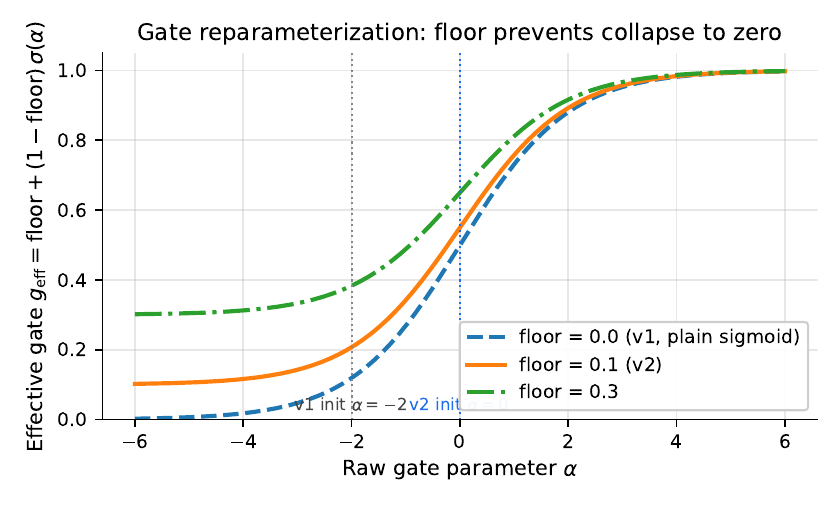
\includegraphics[width=350mm]{gate_reparam.png}};

\node[anchor=north east, font=\itshape\fontsize{22}{28}\selectfont, color=Light,
      text width=350mm, align=right]
    at (-50mm, -320mm)
    {Floor reparameterization. Plain sigmoid (dashed) saturates to zero;
     v2 (solid) is bounded below at 0.1 --- always non-trivial.};

% gate evolution over training
\node[anchor=north east] (evo)
    at (-50mm, -380mm)
    {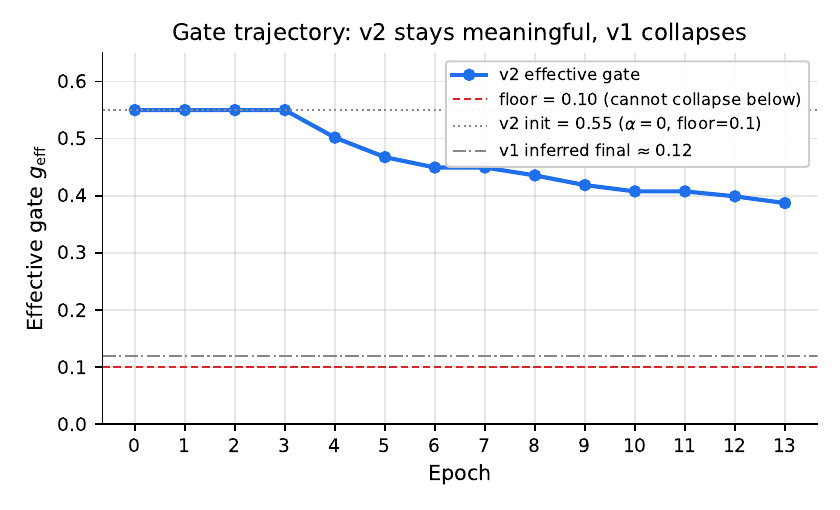
\includegraphics[width=350mm]{gate_evolution.png}};

\node[anchor=north east, font=\itshape\fontsize{22}{28}\selectfont, color=Light,
      text width=350mm, align=right]
    at (-50mm, -610mm)
    {v2 gate stays at $\approx 0.39$ over 13 epochs;
     v1 collapsed to $\approx 0.12$ --- below v2's floor.};

% learning curves
\node[anchor=north east] (lc)
    at (-50mm, -670mm)
    {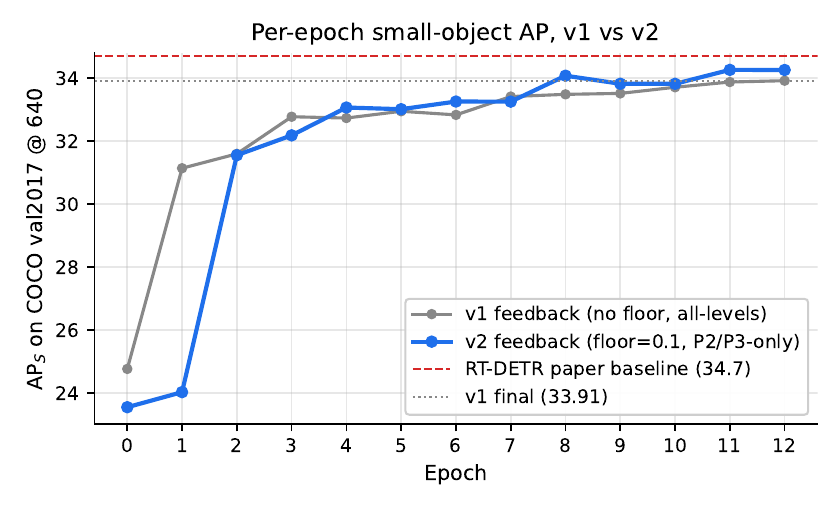
\includegraphics[width=350mm]{learning_curves.png}};

\node[anchor=north east, font=\itshape\fontsize{22}{28}\selectfont, color=Light,
      text width=350mm, align=right]
    at (-50mm, -890mm)
    {v2 (blue) crosses v1's final 33.91 at epoch 8 --- four epochs early.
     Stronger trajectory throughout.};

\end{scope}

% =====================================================================
% Bottom dark band — takeaway + repo
% =====================================================================
\fill[DeepNavy]
    ([yshift=120mm]current page.south west)
    rectangle ([yshift=0mm]current page.south east);

\node[anchor=center, white, font=\bfseries\fontsize{42}{50}\selectfont,
      text width=720mm, align=center]
    at ([yshift=80mm]current page.south)
    {The methodological lesson:};

\node[anchor=center, white!85, font=\itshape\fontsize{34}{40}\selectfont,
      text width=720mm, align=center]
    at ([yshift=40mm]current page.south)
    {An unconstrained sigmoid gate gives the optimizer a costless route to silence
     a new module. A floor on the gate is a one-line structural fix that closes that route.};

% bottom-left author block
\node[anchor=south west, white,
      font=\bfseries\fontsize{28}{34}\selectfont]
    at ([shift={(50mm,30mm)}]current page.south west)
    {Hatem Saadallah \;$\cdot$\; Nour Jennane};

\node[anchor=south west, white!70,
      font=\fontsize{22}{28}\selectfont\ttfamily]
    at ([shift={(50mm,12mm)}]current page.south west)
    {github.com/HatemSaadallah/feedback-augmented-rtdetr};

% bottom-right QR
\node[anchor=south east, fill=white, inner sep=4mm]
    at ([shift={(-50mm,15mm)}]current page.south east)
    {\qrset{height=8cm}\qrcode{https://github.com/HatemSaadallah/feedback-augmented-rtdetr}};

\end{tikzpicture}
\end{document}
